\documentclass{article}
% \url{https://tex.stackexchange.com/q/427775/86}

\usepackage{tikz}

\usetikzlibrary{calligraphy}

\ExplSyntaxOn
\NewDocumentCommand \SPathSplit { m m m m }
{
  \spath_get:nnN {#2} {path} \l__tmpa_tl
  \spath_split_curve:nVNN {#1} \l__tmpa_tl \l__tmpb_tl \l__tmpc_tl
  \spath_clear_new:n {#3}
  \spath_clear_new:n {#4}
  \spath_put:nnV {#3} {path} \l__tmpb_tl
  \spath_put:nnV {#4} {path} \l__tmpc_tl
}
\ExplSyntaxOff

\makeatletter
\tikzset{save as spath/.code={%
    \tikz@addmode{%
      \pgfsyssoftpath@getcurrentpath\spath@tmp@path%
      \MakeSPath{#1}{\spath@tmp@path}%
    }%
  },%
  restore spath/.code={%
    \SPathInfoInto{#1}{minbb}{\spath@tmp@pt}%
    \expandafter\pgfqpoint\spath@tmp@pt
    \pgf@protocolsizes\pgf@x\pgf@y
    \SPathInfoInto{#1}{maxbb}{\spath@tmp@pt}%
    \expandafter\pgfqpoint\spath@tmp@pt
    \pgf@protocolsizes\pgf@x\pgf@y
    \SPathInfoInto{#1}{path}{\spath@tmp@path}%
    \pgfsyssoftpath@setcurrentpath\spath@tmp@path
  },
  heavy line width=.8pt,
  light line width=.1pt,
  line cap=butt
}
\makeatother


%%%%%%%%%%%%%%%%%%%%%%%%%%%%%%%%%%%%%%%%%%%%%%%%%%%%%%%%%%%

% https://tex.stackexchange.com/questions/143070/drawing-randomly-ragged-lines-in-technical-drawings

% irregular line
\usepackage{tikz}
\usepackage{xparse}
\usetikzlibrary{calc}

\NewDocumentCommand{\irregularline}{%
  O     {2mm}   % Amplitude of irregularity. Optional. Default value = 2mm
  m             % First point
  m             % Second point
  D   <> {20}   % Number of peaks. Optional. Default value = 20
}{{%
  \coordinate (old) at #2;
  \foreach \i in {1,2,...,#4}{
    \draw (old) -- ($ ($#2!\i/(#4+1)!#3$) + (0,#1*rand) $) coordinate (old);
  }
  \draw (old) -- #3;
}}


% pencil like
\usetikzlibrary{decorations.pathmorphing}

\newcommand{\none}{
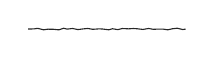
\begin{tikzpicture}[pencildraw/.style={
    black!85,
    decorate,
    decoration={random steps,segment length=1.8pt,amplitude=0.3pt}
    }
]
\draw[pencildraw] (0,1) -- (2,1);
\end{tikzpicture}


% pencilline
\usetikzlibrary{calc,decorations.pathmorphing,patterns}
\pgfdeclaredecoration{penciline}{initial}{
    \state{initial}[width=+\pgfdecoratedinputsegmentremainingdistance,
    auto corner on length=1mm,]{
        \pgfpathcurveto%
        {% From
            \pgfqpoint{\pgfdecoratedinputsegmentremainingdistance}
                      {\pgfdecorationsegmentamplitude}
        }
        {%  Control 1
        \pgfmathrand
        \pgfpointadd{\pgfqpoint{\pgfdecoratedinputsegmentremainingdistance}{0pt}}
                    {\pgfqpoint{-\pgfdecorationsegmentaspect
                     \pgfdecoratedinputsegmentremainingdistance}%
                               {\pgfmathresult\pgfdecorationsegmentamplitude}
                    }
        }
        {%TO  
        \pgfpointadd{\pgfpointdecoratedinputsegmentlast}{\pgfpoint{1pt}{1pt}}
        }
    }
    \state{final}{}
}

\newcommand{\penciline}{
\begin{tikzpicture}[decoration=penciline, decorate]
  \draw[decorate,thick] (0,3) -- (3,3);
\end{tikzpicture}
}   
    

}

%%%%%%%%%%%%%%%%%%%%%%%%%%%%%%%%%%%%%%%%%%%%%%%%%%%%%%%%%%%


%%%%%%%%%%%%%%%%%%%%%%%%%%%%%%%%%%%%%%%%%%%%%%%%%%%%%%%%%%%%%%%%%%%%%

\begin{document}


\begin{tikzpicture}
\pen (0,0);
\clip (1,-5) rectangle (11,1);
\foreach[count=\n] \x in {0,0.05,...,2}{
  \tikzset{every path/.style={blue!\n!red!80},pen colour=blue!\n!red!80}
  \begin{scope}[opacity=.35,transparency group]
  \path[save spath=curve] (0,\x) .. controls (4-\x,-4-3*\x) and (11-2*\x,4-3*\x) .. (12,-5+3*\x);
  \SPathSplit{1/2}{curve}{first}{last}
  \SPathSplit{1/2}{first}{first}{middle}
  \draw[ultra thin, restore spath=first];
  \calligraphy[heavy, restore spath=middle];
  \draw[ultra thin, restore spath=last];
  \end{scope}

  \begin{scope}[opacity=.35,transparency group]
  \path[save spath=curve] (0,\x-1) .. controls (4-\x,\x-2) and (11-2*\x,-4-3*\x) .. (12,-3+3*\x);
  \SPathSplit{3/4}{curve}{first}{last}
  \SPathSplit{3/4}{last}{middle}{last}
  \draw[ultra thin, restore spath=first];
  \calligraphy[heavy, restore spath=middle];
  \draw[ultra thin, restore spath=last];
  \end{scope}

  \begin{scope}[opacity=.35,transparency group]
  \path[save spath=curve] (0,\x-3) .. controls (4-\x,\x-2) and (11-4*\x,-1-4*\x) .. (12,-5+3.5*\x);
  \SPathSplit{1/4}{curve}{first}{last}
  \SPathSplit{2/3}{last}{middle}{last}
  \draw[ultra thin, restore spath=first];
  \calligraphy[heavy, restore spath=middle];
  \draw[ultra thin, restore spath=last];
  \end{scope}


}
  \end{tikzpicture}


%%%%

\none

\begin{tikzpicture}
  \irregularline{(0,0)}{(5,5)}
  \irregularline[1mm]{(1,0)}{(6,5)}
  \irregularline[1mm]{(2,0)}{(7,5)}<100>
\end{tikzpicture}

%%%%%

% example from https://mirror.las.iastate.edu/tex-archive/graphics/pgf/contrib/spath3/calligraphy.pdf

\begin{center}
\tikz \calligraphy[copperplate] (0,0) .. controls +(1,-1) and
+(-1,1) .. ++(3,0) [this stroke style={light,taper=start}] +(0,0) .. controls +(1,-1) and +(-1,1) .. ++(3,0) [this stroke style={heavy}] +(0,0) .. controls +(1,-1) and +(-1,1) .. ++(3,0) [this stroke style={light,taper=end}];
\end{center}

%%%

% https://jan.ucc.nau.edu/ns46/587/TeX/tikz/TikzTutorial.pdf 

\begin{tikzpicture}
	\draw [] 
		(0,0) .. controls (1,.75) and (3,-.5) .. (5.5,0);
	\draw []
		(6,0) .. controls (7,.75) and (9,-.5) .. (11.5,0);
\end{tikzpicture}

\begin{tikzpicture}
	\draw   (0,0) .. controls (1,1) and (3,-1) .. (5.5,0);
	\draw	(6,0) .. controls (7,1) and (9,-1) .. (11.5,0);
\end{tikzpicture}

\begin{tikzpicture}
\draw [dashed ,->]
	(0,0) .. controls (1,1) and (2,-1) .. (3,0);
\draw [densely dotted ,<->]
	(4,0) to [out=90, in=-160]
	node[pos=.6,sloped,above] {$\sum$} (6,0);
\end{tikzpicture}

%%%

\penciline

%%%%%

\end{document}
